%xelatex
\documentclass{article}

\usepackage[T2A]{fontenc}
\usepackage[english,ukrainian]{babel}
\usepackage{fontspec}
\setmainfont{Nimbus Roman}
\usepackage{graphicx}
\usepackage[a4paper,margin=0.5in]{geometry}
\begin{document}

\pagestyle{empty}
\begin{center}

	{\fontsize{14}{24}\selectfont МІНІСТЕРСТВО ОСВІТИ І НАУКИ УКРАЇНИ

	НАЦІОНАЛЬНИЙ УНІВЕРСИТЕТ «ЛЬВІВСЬКА ПОЛІТЕХНІКА»

	Інститут комп'ютерних наук та інформаційних технологій

	}

	\vspace{90.4pt} %120.4+16.1
	\begin{figure}[h]
		\centering
		
\includegraphics[width=6.5cm,keepaspectratio]{../../../lpnu.png}
	\end{figure}

	{\fontsize{18}{29}\selectfont{Звіт}

	{до практичної роботи № 3}

	{З дисципліни}

	{``Дискретна математика''}

	{на тему:}

	{``Обходи графа. Знаходження найкоротшого маршруту за
алгоритмом Дейкстри''}

	}
\end{center}

\vspace{12.1pt} %30.1pt
	{\fontsize{14}{22.4}\selectfont
\begin{flushright}
	\textit{Виконав:}

	\textit{студент групи ПП-14}

	\textit{Мілюхін Олександр}

	\textit{Прийняла:}

	\textit{Ребот Д. П.}
\end{flushright}
\vspace{37.4pt} %100.4
\begin{center}
\textit{Львів-2022}
\vspace{37.4pt} %100.4
\end{center}
	}
%{\fontsize{18}{20.7}\selectfont \textbf{Лабораторна робота №1}}
{\fontsize{14}{16.1}\selectfont
\textbf{Мета роботи:}


Мета роботи – освоїти алгоритми обходу графа вшир та вглиб, навчитися знаходити
найкоротший маршрут за алгоритмом Дейкстри.

\vspace{16pt}
\begin{center}{\textbf{Варіант 12}}\end{center}
\section{Виконати обхід графа методом пошуку вглиб та вшир графа:}
\begin{figure}[h]
	\centering
	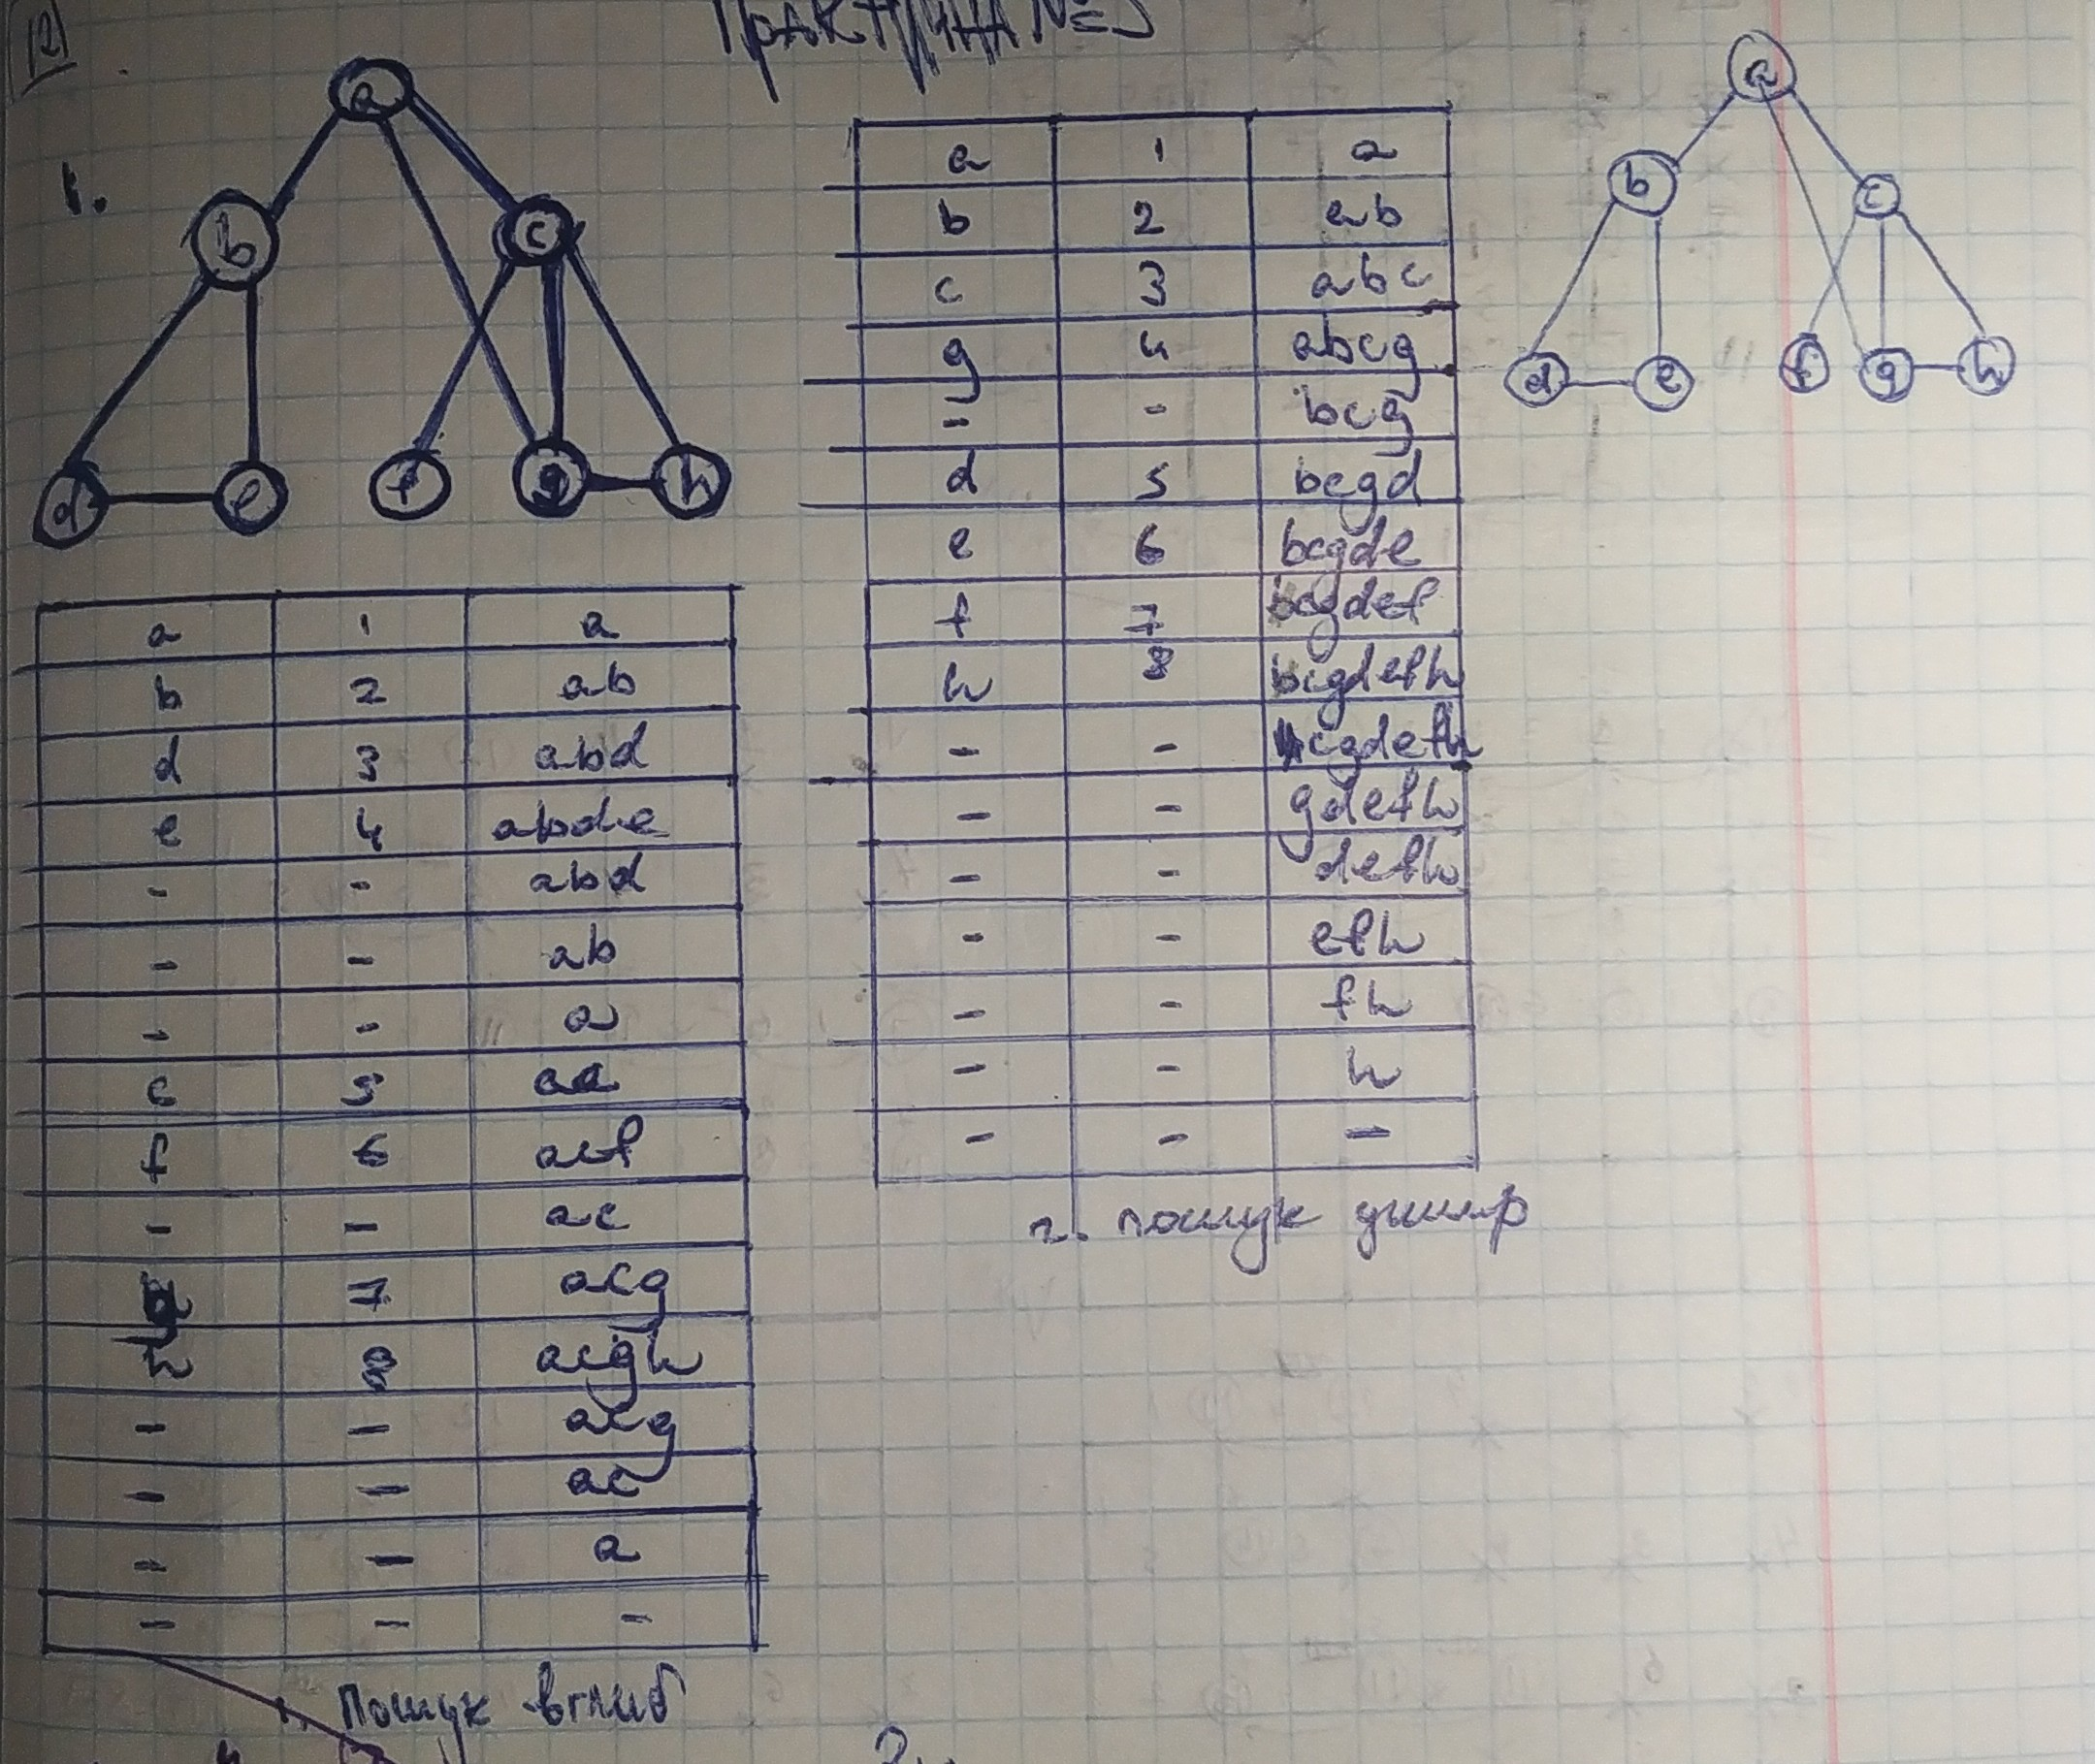
\includegraphics[width=17cm]{pr3.jpg}
%	\caption{}
\end{figure}
\newpage
\section{За допомогою алгоритма Дейкстри знайти найкоротший шлях у графі між парою
вершин V$_0$ i V$^*$:}
\begin{figure}[h]
	\centering
	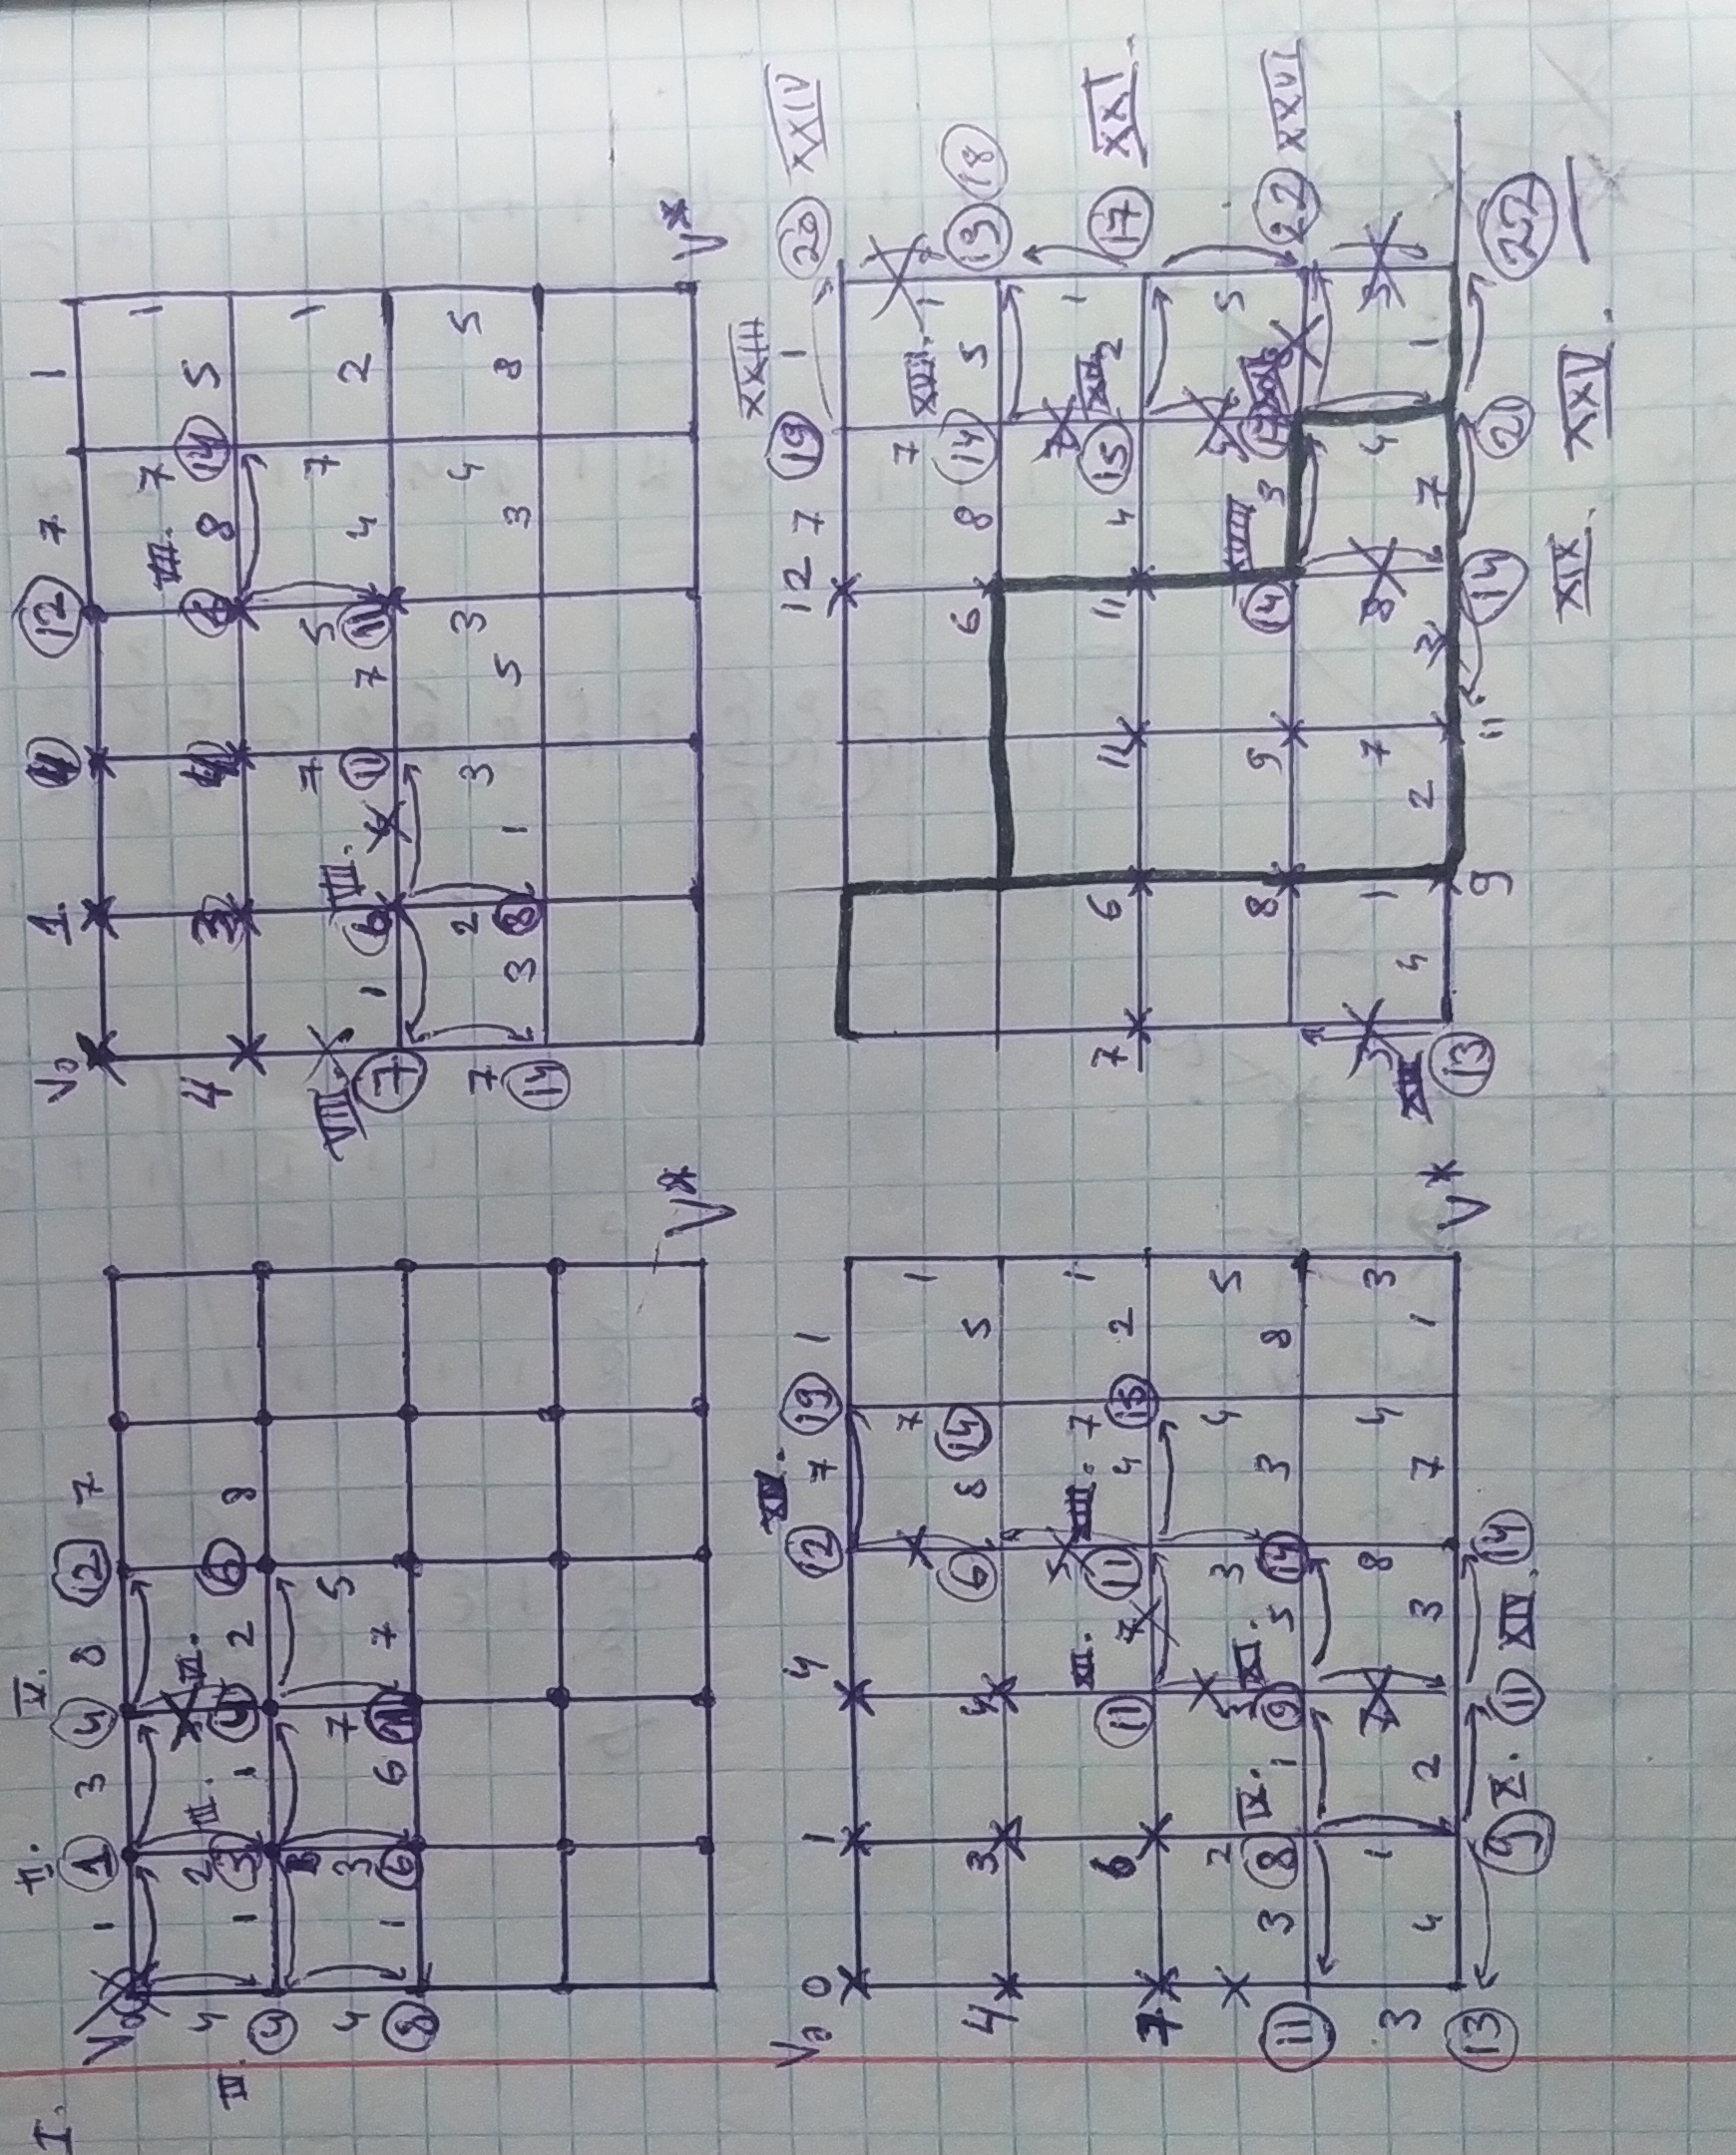
\includegraphics[width=15cm,angle=270]{lol2.png}
\end{figure}

\textbf{Висновок:}

Виконуючи цю роботу, я застосував на практиці
та закріпив свої
знання про методи обходу графа вшир та вглиб,
пошук найкоротшого шляху між вершинами з
використанням алгоритму Дейкстри.

}

\end{document}
